\documentclass[a4paper,12pt]{report}
\usepackage[utf8]{inputenc}
\usepackage{graphicx}
\usepackage{array}
\usepackage{supertabular}
\usepackage{hhline}
\usepackage{siunitx}
\usepackage{hyperref}
\makeatletter
\newcommand\arraybslash{\let\\\@arraycr}
\makeatother
\setlength\tabcolsep{1mm}
\renewcommand\arraystretch{1.3}
\graphicspath{ {images/} }
\title{Computing Practical Project}
\author{Oscar Daniel}
\date{Febuary 2015 }
\begin{document}



\maketitle
\tableofcontents

\chapter{Analysis}

\section{Background and Definition of Problem}
\begin{flushleft}
At Queen Elizabeth Grammar School, pupils in year 13 are taught several calculations for their science subjects. They are tested on these every month or so, after the unit has been taught and students are assumed to understand the topics. Students are set questions during teaching time, however these results are not recorded and sometimes a struggling student may slip under a teacher’s radar.
\\\textbf{Examples of A Level Calculations:}\\
\bigskip
\textbf{Rate of reaction equations}\\

A set of reaction equations used to deduce the rate of a reaction, the concentrations of reactants, their orders and the rate constant: k. \\
A reaction of reactants $A + B \rightarrow D $ where A has the concentration \SI{0.0023}{mol.dm^{-3}} and the power 1. B has the concentration \SI{0.0154}{mol.dm^{-3}}
with the power 2. Whilst the rate of reaction is \SI{0.000045}{mol.s{-1}}.

\emph{An example question.}	\\
\bigskip
\textbf{Standard deviation}\\
 A statistical value that is used ceaselessly in biology.\\
         You and your friends have just measured the heights of your dogs (in millimetres):
         The heights (at the shoulders) are: 600mm, 470mm, 170mm, 430mm and 300mm.
	Find the standard deviation\\
Find out the Mean, the Variance, and the Standard Deviation.\\
Your first step is to find the Mean:
The mean (average) height is 394 mm\\
Now we calculate each dog's difference from the Mean. To calculate the Variance, take each difference, square it, and then average the result:

So, the Variance is 21,704.\\
And the Standard Deviation is just the square root of Variance, so:
Standard Deviation: $\sqrt{21,704}$ = 147.32  = 147 (to the nearest mm)\\


         \emph{ An Example Question}\\
         \bigskip
\textbf{Ideal Gas Equation}\\  A calculation that is used in both chemistry and physics A level.\\
The ideal gas equation is PV = nRT. P is pressure in Pa, V is volume in cubic metres, n is number of moles and T is temperature in degrees Kelvin. R is the ideal gas constant which is measured as 8.314 Joules per Kelvin per Mole.\\
STP = 273K and 100kPa\\
Problem 1: Determine the volume of occupied by 2.34 grams of carbon dioxide gas at STP.\\
Our first job is to rearrange the equation to find V: V = nRT/P\\
Then find moles of ${CO}_{2}$: 2.34/44 =  0.0532\\
Then apply these to the equation.\\
$ (0.0532*8.314*273)/100,000 = 0.0012074921  m^3 $\\
Problem 2: A sample of argon gas at STP occupies 56.2 litres. Determine the number of moles of argon and the mass in the sample.\\
Rearrange to find n: n=PV/RT\\
56.2  litres = 0.0000562 $ m^3 $\\
(100,000*0.0000562)/(8.314*273) = 0.00247607416 moles. $ Ar = 18g/Mole $\\
$ 18*0.00248 = 0.0446g $\\

	\emph{An Example Question}\\
	\bigskip
\textbf{Hardy – Weinberg Equation}\\
A statistical test that is used to estimate the proportions of different genotypes in a population.\\
1. If 98 out of 200 individuals in a population express the recessive phenotype, what percent of the population would you predict would be heterozygotes?
(a) I have given you information on the frequency of the homozygous recessive (or $q^2$). So start by determining q2 and then solving for q.  $ 98/200 =  q^2 = 0.49 $
$\sqrt{0.49}$ = 0.7 = q\\
(b) Now that you have q, you can solve for p. Remember there are only two alleles in the population, so if you add the frequency of the two alleles, you have accounted for all possibilities and it must equal 1. So $ p + q = 1 \text{ Therefore: } p = 1-q = 0.3$\\
(c) Now what is the formula for heterozygotes? Think back to the Hardy-Weinberg equation -- it is dealing with the genotypes of individuals in the population.
$ 2pq = 2*0.3*0.7 = 0.42 $\\
(d) Now that you have figured out the percentage of heterozygotes, can you figure out the percentage of homozygous dominant? Does the percentage of homozygous dominant, heterozygotes and homozygous recessive individuals add up to 100 percent? If not, you have made an error. Those are the only three genotypes possible with only two alleles and a simple dominant and recessive relationship.
$ 1-(0.49 + 0.42) = p^2 = 0.09 \text{ or } 0.3^2 $\\
\emph{An Example Question}
\end{flushleft}


\section{Users and the current system}

Mr Fascione is the head of Science at QEGS.  He focusses on student grades and student support alongside being a teacher.\bigskip

Currently the only way for pupils’ scores from homework to be tracked is by them being entered manually into a spreadsheet after being recorded on paper. There is also no way for pupils to have their problems solved, or explained step by step, other than referring to a text book, which is not interactive. Student feedback is also only monitored for tests, with this system every piece of homework could be used for student support.\bigskip

Pupils can only access a few problems that have been devised by teachers or examiners. These can also be hard for students to grasp, so a program which goes through these at the students’ personal pace would be of great use. Teachers also have no digitally stored questions that can be easily sent to students, they must hand out photocopies and these are always being lost. A computer system would allow work to be set easily, without risk of students losing their things, as well as teachers not losing score sheets.\bigskip

From my feedback and interviews from my end users I have been able to select the appropriate calculations for the computer package to use, and also have a framework to try and emulate, to best please my end user.\\


\section{Feedback Reports}
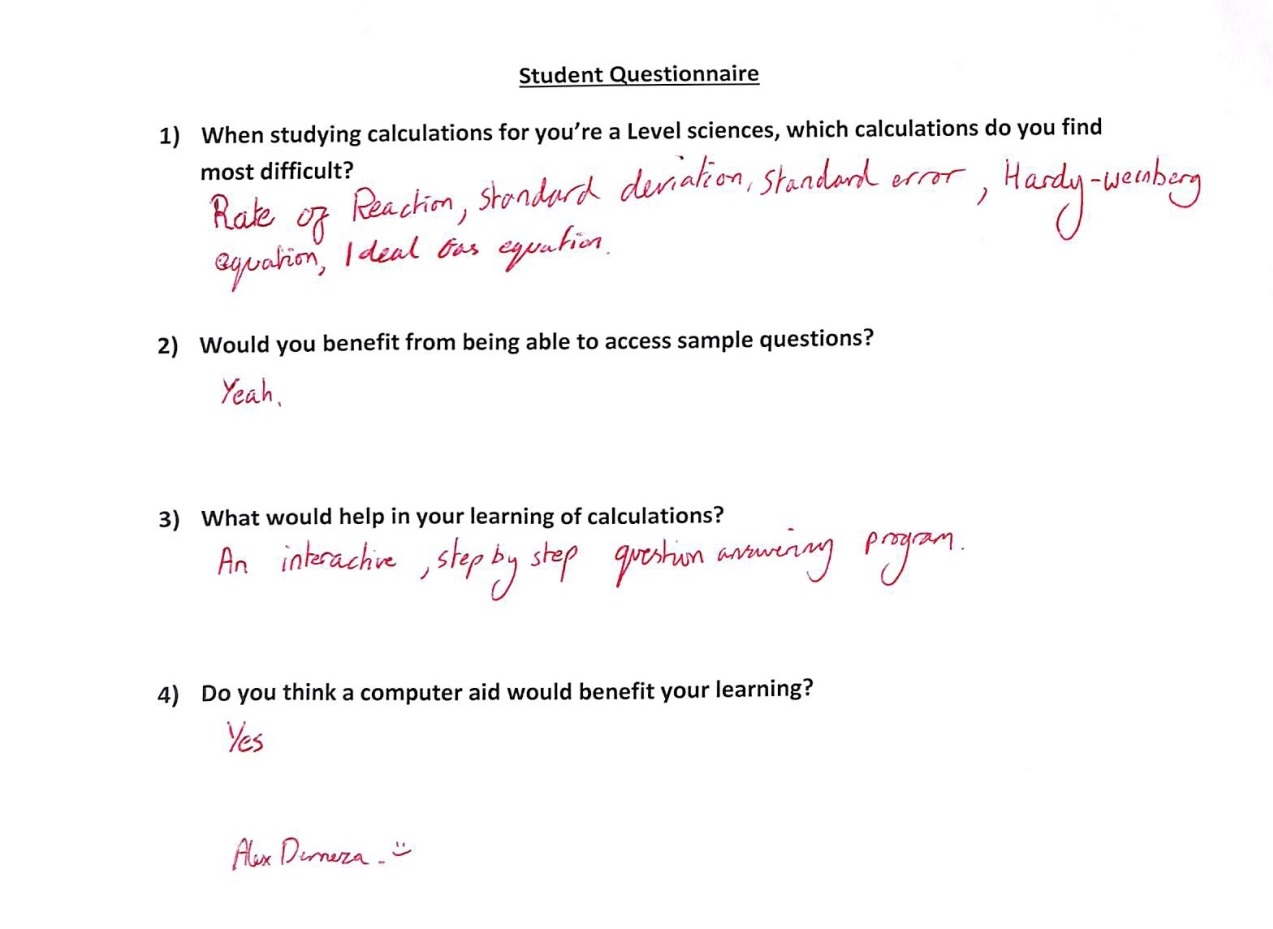
\includegraphics{StudentQuestionnaire}
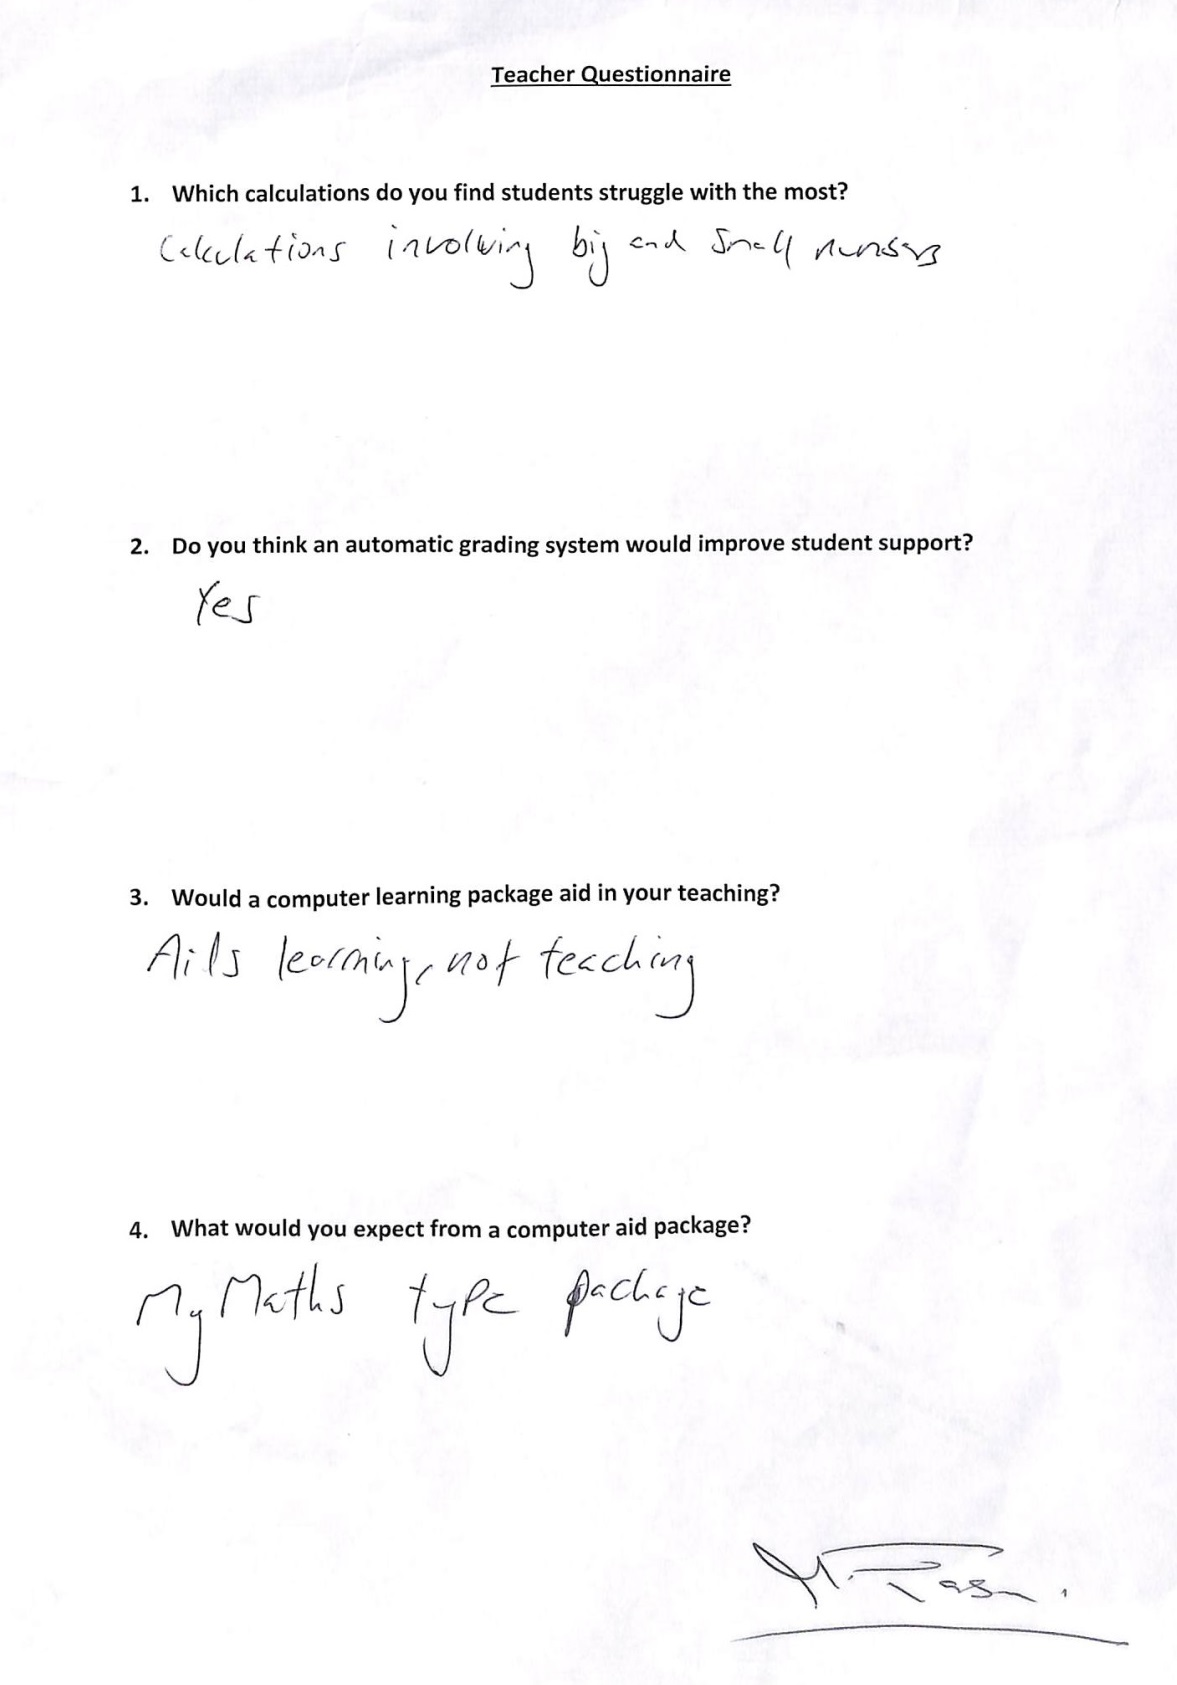
\includegraphics{TeacherQuestionnaire}

\clearpage
\section{Proposed System}        

Pupils will need to be able to input their own problems and have them be solved in a step by step process where they can enter their answer for each step. The program will tell them if they were right and instructing them as to what they should be doing.\\
 They will also be able to store their own problems and solutions in the central database.\\
 Teachers will be allowed to set work to be done and see the scores.\\
 Teachers and pupils will also have unique accounts with teachers having the ability to see pupil scores and set questions. If pupils are having difficulties then they can send a message to the teacher and vice versa. Teachers should be able to make new pupil and teacher accounts and delete old ones.\\
 Allows students and staff to log in.\\
 The program will generate its own questions but may not display questions in the correct format.\\
 Only 100 questions will be stored at once as the memory taken up would be too high.\\
 Pupil accounts would have to be entered in manually as school will not give me access to the student detail database.\\

\section{Objectives}


\textbf{Essential Objectives}\\
\begin{enumerate}
\item Example Based Demonstration – The program should be able to provide a clear demonstration of how any of the equations work, by executing them for the user. It should be able to carry out this demonstration either on data entered by the user, or on data stored within the program/database.
\item Background Explanation Of Problems- The program should be able to give a small amount of detail initially if the student should request it
\item Interactive System allowing Users to Solve Equations – The user should be able to choose to attempt to solve the equations themselves – if this is the case the program should point out (or correct) any mistakes they may have made.
\item Unique User Accounts- Teachers and pupils should have different accounts with different privileges.
\item A System To Allow Users to Input and Store Questions – The users should be able to input their own questions, that the program can solve or walk them through, and have the option to store them.
\item A Database Holding Question Data- the program should run off of a back end database holding around 100 questions in total, which can randomly select a question, or allow a teacher to set specific questions for the pupil to answer.
\item A System For Teachers to set questions and Students Send Feedback – The program should allow teachers to select questions from the database to give to students. Students should be able to send feedback to their teachers.
\item A Database Holding Pupil Performance- Teachers should have access to the questions that pupils answered correctly and incorrectly so that they can monitor their performance and therefore provide support.
\end{enumerate}

\textbf{General Objectives}
\begin{enumerate}
\item Teachers should be able to create or delete user accounts.
\item  A central database should collate all information into a practical form.
\item The program should be self-explanatory and not overly complex for the user.
\item Should use less than 100MB of storage.
\item Grade scores. Highlights students who are below their target grades
\item Allows for students to make comments on problems so the teacher can help them.
\item A log in system with passwords and usernames
\end{enumerate}

\textbf{Acceptable Limitations}\\
\begin{enumerate}
\item  To allow the program to generate questions properly with the correct units would require the use of libraries and a lot more time than I have available.
\item  As my school will not allow me access to the student details database, students must be entered in manually.
\item  Only 100 questions stored at one time to control database size. As there may be hundreds of students inputting questions, the database may have thousands of questions at one time, which would make it cumbersome to use.
\item As the school already has a functioning email system, it would be unnecessary to recreate this system in my project.
\item  As having a function to solve equations could lead to cheating, I will leave this out.
\end{enumerate}

\section{Data Information}
Instead of using an SQL database to store information, as I am using an object oriented system I will use the Pickle function in Python to store my objects and classes as .pickle binary files. This allows for compact storage and easy data storage manipulation within python.

\begin{flushleft}
\tablefirsthead{}
\tablehead{}
\tabletail{}
\tablelasttail{}
\begin{supertabular}{|m{1.5358598in}|m{1.5781599in}|m{1.4483598in}|m{1.5406599in}|}
\hline
\centering Data &
\centering Source &
\centering Destination &
\centering\arraybslash Type\\\hline
Student Name &
Input manually &
Student PICKLE File &
String\\\hline
Student ID &
Generated by Database &
Student PICKLE File &
Integer\\\hline
Student Password &
Input manually &
Student PICKLE File &
String\\\hline
Student Test Scores &
Generated by program &
Student PICKLE File &
Integer and String\\\hline
Student Target Grade &
Input manually &
Student PICKLE File &
String\\\hline
Teacher Name &
Input manually &
Teacher PICKLE File &
String\\\hline
Teacher Password &
Input manually &
Teacher PICKLE File &
String\\\hline
Questions &
Input manually &
Question PICKLE File &
Integer and String\\\hline
\end{supertabular}
\end{flushleft}


\section{Object Orientated Programming Planning}

\begin{flushleft}
\tablefirsthead{}
\tablehead{}
\tabletail{}
\tablelasttail{}
\begin{supertabular}{|m{0.81435984in}|m{1.0191599in}|m{0.8469598in}|m{0.9038598in}|m{2.43586in}|}
\hline
Access Type &
Field Name &
Field Type &
Initial Value &
Description\\\hline
Private &
Pupil Data &
Strings and Integers &
{}- &
The data associated with a student. Contains information about them, i.e. form group.\\\hline
Private &
Question Data &
Strings and Integers &
{}- &
Data contained in the question object. Gives format for insertion into program.\\\hline


\end{supertabular}
\end{flushleft}

\chapter{Design}
\section{Navigation}

\begin{itemize}
\item Log in menu

\begin{itemize}
\item Main Menu

\begin{itemize}
\item Set Questions *
\item Select Student/s*
\item Select Question/s*
\item See Set Work \^{}
\item Attempt Set Questions\^{}
\item Practice
\item Finding K Questions
\item Select question from list / Randomly
\item Finding Rate Of Reaction Questions
\item Select question from list / Randomly
\item Messages

\begin{itemize}
\item Open Messages
\item Create Message

Recipient
Content
\end{itemize}
\end{itemize}
\end{itemize}
\end{itemize}
Etc.

\section{Validation}


\bigskip

\begin{flushleft}
\tablefirsthead{}
\tablehead{}
\tabletail{}
\tablelasttail{}
\begin{supertabular}{|m{0.7156598in}|m{0.69835985in}|m{2.19556in}|m{0.8288598in}|m{1.5691599in}|}
\hline
Field Name &
Validation Checks &
Description &
Error Message &
Data Input\\\hline
Gender &
Listed Data (``M'', ``F'') &
Only allow M or F &
Please select legal gender. &
Radio Button\\\hline
Name &
Presence, Data Type. &
Only allow names with letter characters, apostrophes or hyphens, make sure a name is present. &
Please enter a name. / Please remove invalid characters from field. &
F0rd Pr3f3ct\\\hline
Form Group &
Presence, Listed Data. &
Allow only listed form groups. &
Please select a form group from the list. &
Drop Down\\\hline
Password &
Presence, correct password format. &
Any string of ascii characters, including numbers and special characters. &
Please enter a valid password. &
Slartibartfast\\\hline
Target Grade &
A, B, C, D, E, F or U &
A single ASCII upper case character. &
Please enter a target grade. &
A\\\hline
Parent Email &
Correct email format. &
{}String.string'@'string.'string &
Please enter a valid email address. &
myEmail@email.net

~
\\\hline
\end{supertabular}
\end{flushleft}

\bigskip


\bigskip

The student class which I have designed incorporates all of the information above, apart from email and gender as it is going to be used at an all-boys school which stores parental contact information securely. Therefore those two data fields would not be appropriate to store in my program. The pupil class accepts input in this format: ( studentid, password, forename, surname, middlename, age, form, targetgrade, questionsanswered, questionstoanswer, answeredcorrectly)


\bigskip

The questionsanswered, questionstoanswer and \ answeredcorrectly values are worked out by other functions in the program and are set to 0 when a new student is created.

To track a students' performance, when they answer questions the \ percentage() \ \ findgrade() functions take their answered questions and find out if they are keeping to their current target grade.
\section{Overall System Design}


\bigskip


\bigskip

\begin{flushleft}
\tablefirsthead{}
\tablehead{}
\tabletail{}
\tablelasttail{}
\begin{supertabular}{|m{1.6566598in}|m{1.5955598in}|m{1.6011599in}|m{1.6240599in}|}
\hline
Input &
Process &
Storage &
Output\\\hline
Question Data &
Store Question &
Question Pickle &
Question stored successfully.\\\hline
Question Data &
Answer Question &
Question Pickle &
Question Answer.\\\hline
Student Data &
Add Student &
Pupil Pickle &
Pupil Data stored successfully.\\\hline
Question ID, Student ID &
Set Question &
Pupil Pickle &
Questions sent to Pupil\\\hline
Student Answer &
Answer Question &
Retrieve from answer box in window, check answer. Record if wrong or right. Send to pupil pickle. &
Question answered in/correctly.

OR\newline
Answer Sent.\\\hline
Student/Teacher Password &
Log In &
Retrieve from Pupil / Teacher pickle &
Logged in as ``person''\newline
OR

Username password combination is incorrect.\\\hline
\end{supertabular}
\end{flushleft}

\bigskip


\bigskip

\section{Record Structure}


\bigskip

I plan to use pickle tool to store my objects as binary files.

The pickle module implements binary protocols for serializing and de-serializing a Python object structure. ``Pickling'' is the process whereby a Python object hierarchy is converted into a byte stream, and ``unpickling'' is the inverse operation, whereby a byte stream (from a binary file or bytes-like object) is converted back into an object hierarchy.

Pickle accepts inputs in this format: \ \ pickle.dump(obj, file, protocol,)

As an example: \ 
\bigskip

class container():

\ \ \ \ def \_\_init\_\_(self, name):

\ \ \ \ \ \ \ \ self.objects = []

\ \ \ \ \ \ \ \ self.name = name


\bigskip

\ \ \ \ def sayName(self):

\ \ \ \ \ \ \ \ return self.name


\bigskip

\ \ \ \ def listObjects(self):

\ \ \ \ \ \ \ \ for thing in self.objects:

\ \ \ \ \ \ \ \ \ \ \ \ print (thing.sayName())


\bigskip

\ \ \ \ def addObject(self,item):

\ \ \ \ \ \ \ \ self.objects.append(item)


\bigskip


with open('data.pickle', 'wb') as f:

\ \ \ \ \ \ \ \ \ \ \ \ \ \ \ \ \ \ \ \ \ \ \ \ \ \ \ \ \ \ \ pickle.dump(box, f, pickle.HIGHEST\_PROTOCOL)


\bigskip

\^{} Stores class and instance as a binary file (.PICKLE)


\bigskip


\bigskip

with open('data.pickle', 'rb') as f:

\ \ \ \ The protocol version used is detected automatically, so we do not have to specify it.

\ \ \ \ box = pickle.load(f)


\bigskip

\^{} Reads in the information from the file and decodes it.


\bigskip


\bigskip

\section{Data Transformation}


\bigskip


\bigskip
\begin{flushleft}
\textbf{Hardy - Weinberg}

To find the value of 2pq, the number of heterozygotes, we must find q and p. We are given a means of finding q\^{}2 in the question:
\end{flushleft}
\ recessiveInpop = ((totalpop * percentageReccessive) / 100) \ \# unrounded. Makes a percentage of the population have recessive alleles.

\ \ \ \ \ \ \ \ q\_sqrdaspop = Round\_To\_n(recessiveInpop, 1) \ \# now rounded

\ \ \ \ \ \ \ \ qsqrd = Round\_To\_n(q\_sqrdaspop / totalpop, 3) \# Finds q squared as a decimal.

\ \ \ \ \ \ \ \ q = Round\_To\_n(math.sqrt(qsqrd), 3) \# finds the number of reccessive alleles and rounds

\ \ \ \ \ \ \ \ p = Round\_To\_n(1 - q, 3) \#finds the number of dominant alleles and rounds

\ \ \ \ \ \ \ \ psqrd = Round\_To\_n(p * p, 3) \#finds the number of homozygous dominant

\ \ \ \ \ \ \ \ pq = Round\_To\_n(p * q, 3) \# finds heterozygotes\\
\begin{flushleft}

\textbf{Find k}

To find the rate constant k, we take the values the student has been given, place them in the reaction class and send those variables to a function that solves the equation. Then format the answer correctly.
\end{flushleft}

\begin{verbatim}


def rateEquation(myReaction):

intermediary = (pow(myReaction.conc\_of\_A,
 myReaction.order\_of\_A)* 
 (pow(myReaction.conc\_of\_B, myReaction.order\_of\_B)))

myReaction.rateOfReeac intermediary
\end{verbatim}
\ \ \ \ print((format\_e(myReaction.k)))


\ \ \ \ return float(myReaction.noOfMoles)


\bigskip


\bigskip


\bigskip

\section{Security and Integrity}


\bigskip

As Python is an interpreted language, students could in theory open it as a text file. An easy way around this would to use the current controls to not allow students access to the program files. However the program requires read write access to files in order to work. \ However data can be backed up to a secure location once a week. As the files are very small, each time the data is backed up it can be assigned a date


\bigskip


\bigskip


\bigskip

\section{Prototype}


\bigskip

I showed my end user an initial skeleton program that I had created. I responded to their requests and added a function to give the user an option to immediately have another question also, when their answer is incorrect then they are told it was incorrect and are asked to try again. With further testing I thought the user should be able to have the program to take them through the problem, as it is only a practice.\\
\textbf{Command Line Prototype Code}
\begin{verbatim}

author = 'Oscar'
import random
import decimal

def getChoice():
    choice = (input("Please choose an option. "))

    if choice == "1":
        print("  ")
        loadQuestion()
    if choice == "2":
        pass
    if choice == "4":
        pass
    return (choice)


def menu():
    choice = 0


    while choice != "q":
        print("1.Do a practice K question.")
        print("2.See a K example. ")
        print("3. Find units of K. ")
        print("4. Calculate the initial rate of reaction.")
        print("Press q to quit. ")
        choice = getChoice()
        
        
        def format_e(n):
            a = '%E' % n
            return a
        
        
        class findKreaction():
            def __init__(self, conc_of_A, conc_of_B,
             order_of_A, order_of_B, rateOfReaction):
                self.conc_of_A = conc_of_A
                self.conc_of_B = conc_of_B
                self.order_of_A = order_of_A
                self.order_of_B = order_of_B
                # self.rateNumber = rateNumber
                # self.rateExponent = rateExponent
                self.rateOfReaction = rateOfReaction
                self.noOfMoles = (order_of_A + order_of_B)
                
                
            def walk_throughK(self):
                print("To calculate the rate constant, k, we must first 
		 multiply the concentrations of our reactants together."
                      "However the concentrations must be raised to the power
		 of their orders."
                      "The concentrations of A and B are", self.conc_of_A, "and",
		 self.conc_of_B, "respectively."
                      "The order of A is", self.order_of_A, "and the order of B is",
		 self.order_of_B, ".")
                print("This means our intermediary value is", self.intermediary, "."
                      "We then divide our rate of reaction by this number. The reate
		 of reaction is", self.rateOfReaction,".")
                print("This equals", self.k)
                print("Next we must find the units of
                 k")
                print("To find the units of k we must cancel the number of moles
        
        per dm cubed on both sides of the equation. "
                      "We do this by adding the powers of the two reactants 
                      and putting them into the formula: mol^-x dm^+x*3.
                       Where x is the powers added together minus 1."
                      "Unless the number of moles is
                       one, then there are no units.")
                if self.noOfMoles > 1:
                    x = int((self.noOfMoles) - 1)
        
                    print("The units are mol^-", x, "dm^+", 3 * x, "s^-1")
                else:
                    print("No units")        
                
        
        
            def findK(self):
                n = 0
                self.intermediary = pow(self.conc_of_A, self.order_of_A) *
                (pow(self.conc_of_B, self.order_of_B))
                self.k = self.rateOfReaction / self.intermediary
                correct = False
                print("The conc of reactant A is ", self.conc_of_A, "moldm^-3.
                The conc of B is", self.conc_of_B, "moldm^-3")
                print("The order of A is ", self.order_of_A, "and the order of B
                is", self.order_of_B)
                print("The rate of reaction is", self.rateOfReaction)
                while correct == False:
                    k = self.k
                    k = ("%.3G" % (k))
                    
        
                    studentAnswer = input("Enter in your value of k
                    to 3 sig fig: ")
                    if studentAnswer == k:
                        correct = True
                        print("Well done, that was correct!")
                        another = input("Would you like to try again? y/n")
                        if another == "y":
                            print("  ")
                            loadQuestion()
                        if another == "n":
                            print("Goodbye!")
                    if studentAnswer != k:
                        n += 1
                        print("Sorry that's not right, try again.")
                        if n > 2:
                            walkthrough = input("Would you like a walk-through? 
                           	 y/n")
                            if walkthrough == "y":
                                print("  ")
                                findKreaction.walk_throughK(self)
                        
                            
        
        
            def findunitsofK(self):
                print("To find the units of k we must cancel the number of moles 
                per dm cubed on both sides of the equation. "
                      "\We do this by adding the
                       powers of the two reactants and
                       putting them into the formula: "
                      "\nmol^-x dm^+x*3. Where x is
                       the powers added together minus 1."
                       "\nUnless the number of moles is one, then
                        there are no units.\n ")
                if self.noOfMoles > 1:
                    x = int((self.noOfMoles) - 1)
        
                    print("The units are mol^-", x, "dm^+", 3 * x, "s^-1")
                else:
                    print("No units")
        
        
                    # def getRateOfReaction(self):
                    # rateOfReaction = self.k*(pow(10,self.rateExponent))
                    # return rateOfReaction
        
        
        def loadQuestion():
            Q1 = findKreaction(0.4, 0.4, 2, 1, 0.00000585)
            Q2 = findKreaction(0.2, 0.3, 1, 2, 0.0000657)
            Q3 = findKreaction(0.2, 0.3, 1, 2, 0.0000257)
            Q4 = findKreaction(0.2, 0.3, 1, 2, 0.0000457)
            Q5 = findKreaction(0.2, 0.3, 1, 2, 0.0000127)
            Q6 = findKreaction(0.2, 0.3, 1, 2, 0.0100687)
            Q7 = findKreaction(0.2, 0.3, 1, 2, 0.0000757)
            Q8 = findKreaction(0.2, 0.3, 1, 2, 0.0000357)
            Q9 = findKreaction(0.2, 0.3, 1, 2, 0.0000257)
            Questions = [Q1, Q2, Q3, Q4, Q5, Q6, Q7, Q8, Q9]
            x = random.randrange(9)
            y = Questions[x]
            findKreaction.findK(y)
            # findKreaction.findunitsofK(y)
        
        
        menu()
\end{verbatim}
\clearpage
\textbf{Screenshots of CLI Prototype:}\\
\bigskip
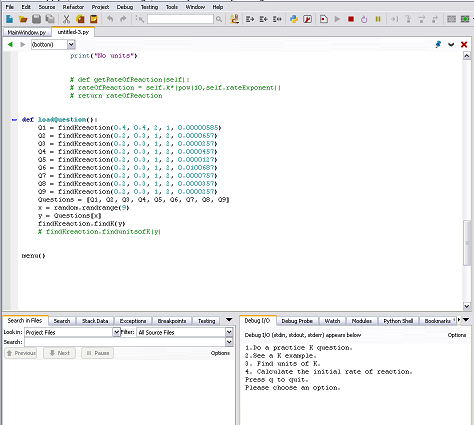
\includegraphics{CLI01}\\
\emph{CLI Main Menu}\\
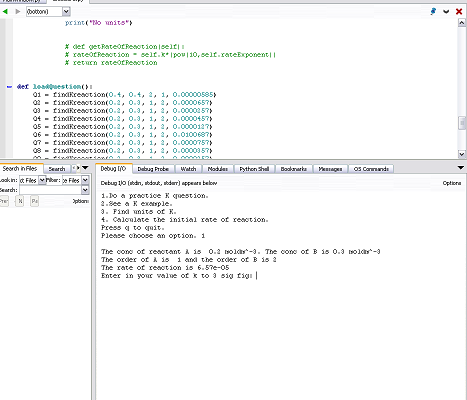
\includegraphics{CLI02}\\
\emph{Attempting a question in CLI}\\
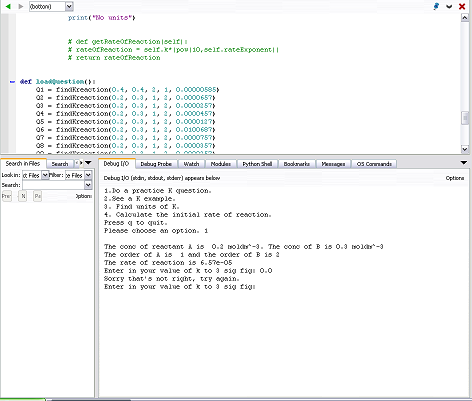
\includegraphics{CLI03}\\
\emph{Entering an incorrect answer}\\
\bigskip

After this I decided that if the student was only practising questions, they should not use up questions that teachers are marking them on. Therefore I created a function that generates random numbers, in a specific range, and rounds them to suit the question. This way, a student will never have encountered the questions they would be assessed on.

\begin{verbatim}


def generateK():
    sig = 3
    
    
    concofa = random.uniform(0.001, 0.9)
    concofA = round(concofa, sig-int(floor(log10(concofa)))-1)
    concofb = random.uniform(0.001, 0.9)
    concofB = round(concofb, sig-int(floor(log10(concofb)))-1)
    orderofA = random.randrange(1,3)
    orderofB = random.randrange(1,3)
    rate = random.uniform(0.00000001, 0.0009)
    rateofreaction = round(rate, sig-int(floor(log10(rate)))-1)
    y = findKreaction (concofA, concofB, orderofA, orderofB, rateofreaction)
    return y
\end{verbatim}
\begin{flushleft}

This generates the numbers for the equation, creates a class using them, then returns it to the main program.
\par
After consulting my end user again, and by using their request of something “MyMaths”-esque, I have implemented a GUI into my design using PyQt, which is event driven. This improves the ease of use of the program and also makes it more user friendly for people who do not use command line regularly.

\textbf{GUI Prototype}\\
To prototype the GUI I hand drew some of my windows and annotated functions:
\end{flushleft}

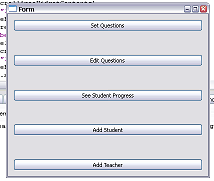
\includegraphics{MainMenuOld}\label{Old Main Menu}\\
\emph{Early teacher main menu}\\
\bigskip
I have also made a form window for the input of new users to the system. This window sends its' variables to a function which adds the new student and repickles the list. This function is only available to teacher accounts. They can also create new teacher accounts in a similar manner.
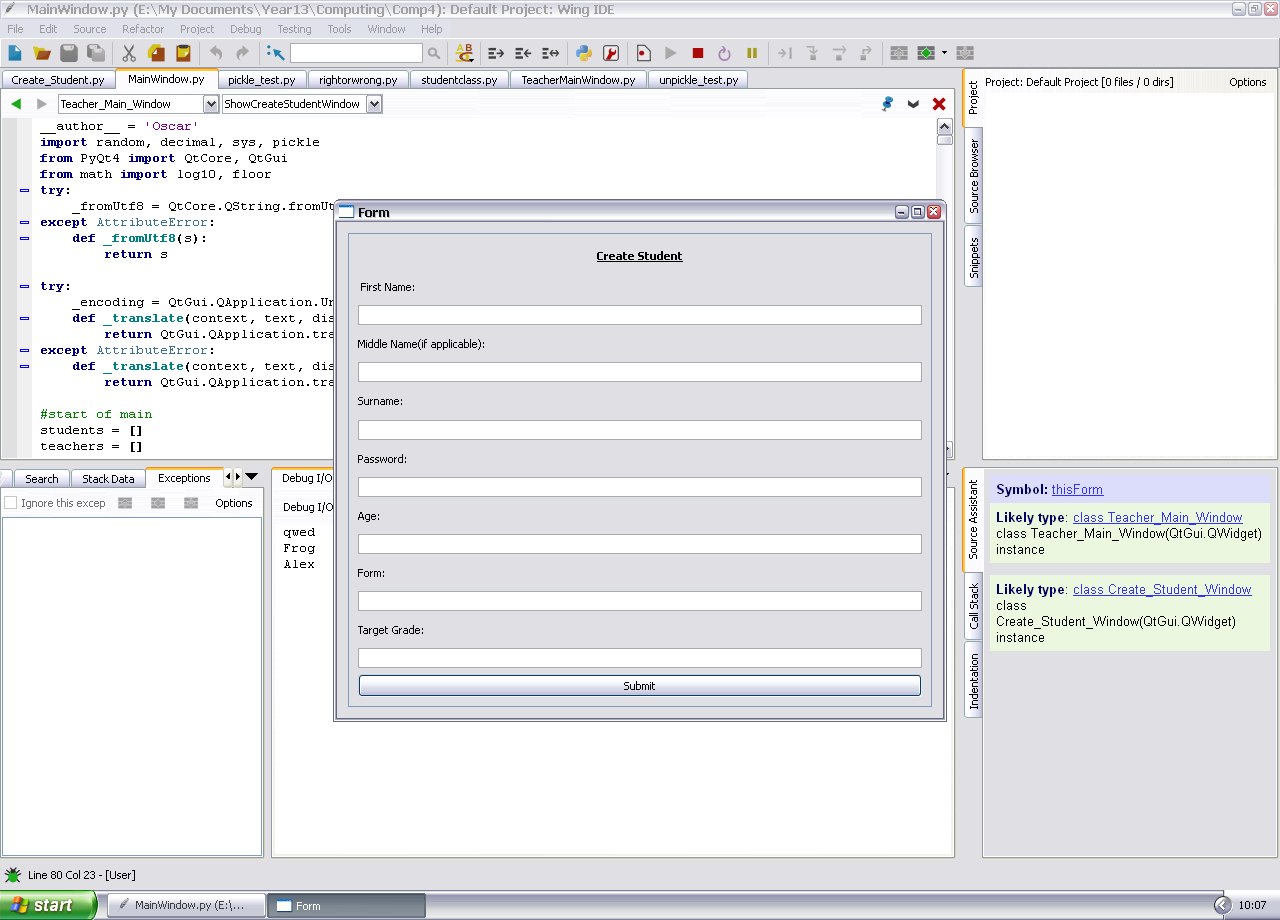
\includegraphics{CreateStudent}\\
\emph{The initial create student window}\\
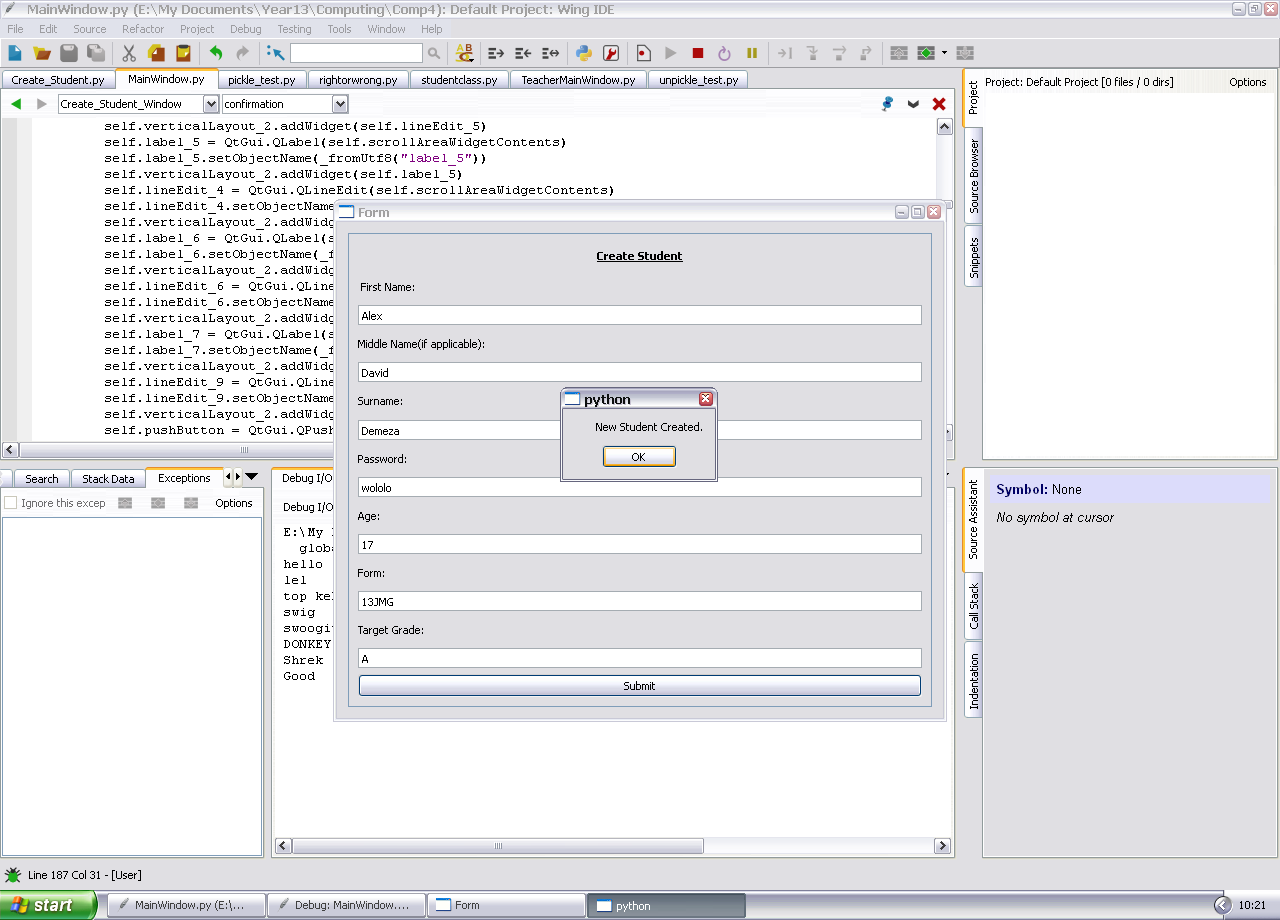
\includegraphics{CreateStudent2}\\
\emph{An account being created}\\
\end{document}